\section{Introduction}

\subsection{Contributions}

\begin{frame}[label=contribs]{Contributions}
  \begin{columns}[t]
    \column{.36\textwidth}
    \begin{block}{Preliminary exam}
      Two approaches to \alert<1>{formal verification of memory usage for binaries}

      \hyperlink{floyd}{\beamerskipbutton{Floyd-style}}
      \hyperlink{hoare}{\beamerskipbutton{Hoare-style}}
    \end{block}

    \pause

    \column{.55\textwidth}
    \begin{alertblock}{Novel contributions: \glsxtrfull{cfr}}
      \begin{outline}
        \pause
        \1 Formally verified disassembly
        \pause
        \1 \Glsxtrfullpl{eicfg} % have to use explicit first as it technically got used on the first slide
      \end{outline}
    \end{alertblock}
  \end{columns}
\end{frame}

\begin{lrbox}\lstbox % neither \sbox nor \savebox works for listings
  \begin{lstlisting}[style=x64,gobble=4,basicstyle=\small\ttfamily]
    cmp eax,c3
    ja  1c
    mov eax,DWORD PTR [eax*4+a]
  \end{lstlisting}
\end{lrbox}
\begin{frame}{Contribution \#3: Formally Verified Disassembly}{Key Points}
  \begin{columns}
    \column{.45\textwidth}
    \begin{outline}
      \1 Disassembly based on \alert{invariants}
        \2 vs.\ heuristics
      \1 \alert{Overapproximative}
        \2 i.e.\ \alert{sound}
    \end{outline}

    \pause
    \rotatebox{-10}{\usebox\lstbox}

    \column{.45\textwidth}
    \begin{example}[Jump Table Invariant]
      \tikzstyle{inv}=[]
      \only<3->{
        \tikzstyle{inv}=[draw,ellipse,red,thick] % inner sep=0pt, <- what does this even do?
      }
      \begin{tikzpicture}[vertex/.style = {circle,draw,minimum size=0.7cm},->]
        \node[vertex]    (b)   at (3,-.5)    {};
        \node[draw=none] (120) at (1.6,-1.5) {};
        \node[draw=none] (121) at (2.3,-1.5) {};
        \node[vertex]    (122) at (3,-2)     {};
        \node[draw=none] (123) at (3.7,-1.5) {};
        \node[draw=none] (124) at (4.4,-1.5) {};

        \node[right,inv] at (3.4,-.45) {$
          \reg{eax} < \mathtt{0xc3}
          $};

        \node[right] at (3.4,-2) {$
          \reg{eax} == a_\mathtt{jt}
          $};

        \draw [overlay,decorate,decoration={brace,amplitude=10pt,mirror},xshift=-4pt] (6,-1.75) -- (6,-.5) node [black,midway,xshift=1.4cm] {
          \begin{tabular}{l}
            up to $\mathtt{0xc3}$\\
            edges: one\\
            per read\\
            value
          \end{tabular}
        };

        \draw[dotted] (b)   to (120);
        \draw[dotted] (b)   to (121);
        \draw         (b)   to (122);
        \draw[dotted] (b)   to (123);
        \path[dotted] (b)   edge node [right,xshift=0.2] {\inlineasm{mov}} (124);
      \end{tikzpicture}
    \end{example}
  \end{columns}
\end{frame}

\begin{frame}{Contribution \#4: Exceptional Interprocedural Control Flow Graphs}{Improvement on the state of the art}
  \centering
  \tikzstyle{backdraw}=[< draw] % Had to reenable bEnd1's ability to draw outgoing edges here as setting it on the edge itself didn't work.
  % Trying to use \only/\uncover/etc. with the graph paths directly doesn't work so need to mess with the styles
  \only<1>{
    \tikzstyle{unwind}=[draw=none]
    \tikzstyle{bad}=[]
    \tikzstyle{good}=[]
    \tikzstyle{backdraw}=[]
    \alert{Regular \glsxtrfull{cfg}}
  }
  \only<2>{\alert{Exceptional interprocedural \glsxtrshort{cfg}}}
  \begin{tikzpicture}
    \graph[
    grow down=1.25cm,
    branch right=1.5cm,
    nodes={draw,ellipse,font=\ttfamily}
    ]{
      foo -> fEnd1/""[ret],
      foo -> "" -> {fEnd1, fEnd2/""[ret]}, % more compact this way
      foo'[landing] -> fEnd'/""[ret],

      bar -> {b1/"", bEnd1/""[ret,< draw=none]} -> {b2/"", bEnd2/""[ret]},
      b2 -> {bar[> bend left], bEnd2},
      b1 -> bEnd2, % necessary due to group/chain interactions
      bar'[landing] -> bEnd'/""[ret],

      {[grow down=1.25cm, branch right=1.5cm]
        {main[circle], catch[landing]} -> {
          callSite/""[diamond],
          ""[at=(0:-.5)],
          ""[ret, bad, at=(0:-1), < draw=none]
        } -> ""[ret,good],
      };

      callSite ->[interproc] foo;
      callSite ->[interproc] bar;

      fEnd1 ->[interproc] callSite;
      bEnd2 ->[interproc] callSite;

      fEnd2 ->[unwind] foo'; fEnd' ->[unwind] catch;
      bEnd1[backdraw] ->[unwind] bar'; bEnd' ->[unwind] catch;
    };
  \end{tikzpicture}
\end{frame}

\subsection{Motivation}

\begin{frame}{Why static binary analysis?}
  \tikzset{every node/.style=draw,->}
  \begin{columns}
  \column{.3\textwidth}
  \begin{block}{Static}
    \centering
    \pause
    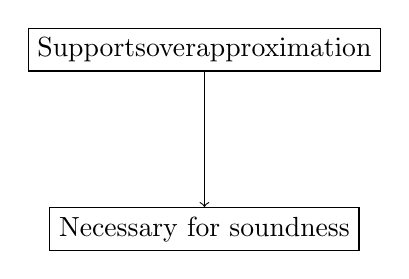
\begin{tikzpicture}
      \node (a) {\makecell{Supports\\\alert{overapproximation}}};
      \pause
      \node [below=2cm] (b) {\makecell{Necessary for \alert{soundness}}};
      \draw (a) -- (b);
    \end{tikzpicture}
  \end{block}

  \column{.58\textwidth}
    \begin{block}<4->{Binary} % Using + wasn't working right; this setup doesn't preserve positioning the way I want but it least puts everything on the right slides
      \centering
      \begin{tikzpicture}
        \node<5-> (a) {Analysis w/o source};

        \node<6-> [below left=.5cm of a] (b1) {Legacy progs};
        \draw<6-> (a) -- (b1);

        \node<7-> [below=.5cm of a] (b2) {Reverse eng.};
        \draw<7-> (a) -- (b2);

        \node<8-> [below right=.5cm of a] (b3) {\makecell{No compiler\\in \glsxtrshort{tcb}}};
        \draw<8-> (a) -- (b3);
      \end{tikzpicture}
    \end{block}
  \end{columns}
\end{frame}

\begin{frame}{Why \glsxtrlong{cfr}?}
  \centering
  \begin{tikzpicture}[every node/.style={draw,ellipse},->]
    \node (prelim) {No indirection in prelim};
    \pause
    \node[below right=2cm] (how) {How to handle?};
    \draw (prelim) -- (how);
    \pause
    \node[below left=2cm of how] (cfr) {Need \gls{cfr}!};
    \draw (how) -- (cfr);
  \end{tikzpicture}
\end{frame}

\begin{frame}[fragile]{Why exceptional \gls{cfr}?}
  \begin{columns}[t]
    \column{.29\textwidth}
    \begin{block}{Error handling in \gls{c}}
      \begin{lstlisting}[gobble=8]
        #include <errno.h>
        int unim(int* x) {
         return ENOSYS;
        }
        int main(void) {
         int x;
         int e=unim(&x);
         if (e) return e;

         return x;
        }
      \end{lstlisting}
    \end{block}

    \column{.67\textwidth}
    \begin{block}{Error handling in \gls{cpp}}
      \begin{lstlisting}[gobble=8]
        #include <system_error>
        int unimp() {
         auto a=std::errc::function_not_supported;
         auto b=std::make_error_code(a);
         throw std::system_error(b);
        }
        int main() {
         return unimp();
        }
      \end{lstlisting}
    \end{block}
  \end{columns}
\end{frame}

\begin{frame}{Novelty Restated}
  \begin{columns}
    \column{.4\textwidth}
    \begin{block}{Formally Verified Disassembly}
      \begin{outline}
        \pause
        \1 Existing disassemblers \alert{unsound} % they make guesses or are not fully overapproximative
        \pause
        \1 \LARGE \alert{We are sound!}
      \end{outline}
    \end{block}

    \pause

    \column{.5\textwidth}
    \begin{block}{\Glsxtrshortpl{eicfg}}
      \begin{outline}
        \pause
        \1 Off-the-shelf \alert{disassemblers, decompilers} do not model \alert{exception unwinding}
        \begin{center}
          
\includegraphics[width=1cm]{GHIDRA_1}
          \hspace{1cm}
          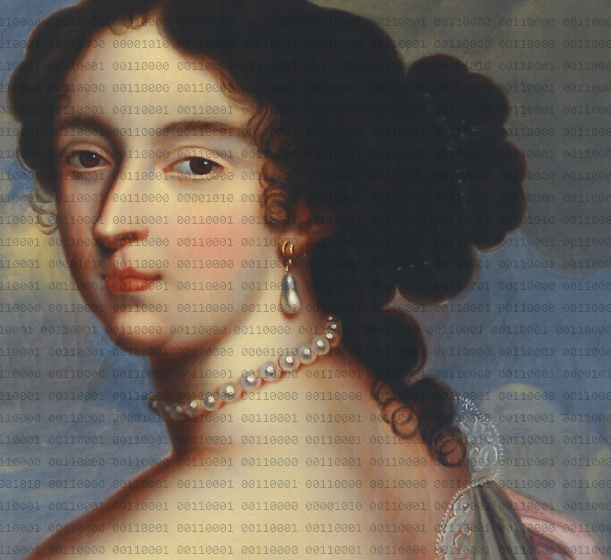
\includegraphics[width=1cm]{ida}
          \hspace{1cm}
          
\includegraphics[width=1cm]{ninja}
        \end{center}
        \pause
        \1 \LARGE \alert{We do!}
      \end{outline}
    \end{block}
  \end{columns}
\end{frame}
